\chapter{Seitenkanalangriffe}
\label{sec:seitenkanalangriffe}
Lange wurden in der Kryptographie die einzelnen Komponenten als Black
Box betrachtet. Man ist davon ausgegangen, dass eine solche Komponente
lediglich definierte Eingaben, wie z.B. Klartext und Schlüssel, bekommt,
um daraus eine definierte Ausgabe zu berechnen. Praktisch kommen jedoch
weitere Eingaben (Strom), weitere Ausgaben (elektromagnetische
Abstrahlung) sowie interne Zustände (und dadurch andere Laufzeiten)
hinzu, die einem Angreifer Informationen über das Geheimnis der
Komponente liefern können. Es gibt eine ganze Reihe solcher
\emph{Seitenkanäle}, die Informationen nach außen tragen
können. Beispiele hierfür sind:
\begin{itemize}
\item Stromverbrauch
\item Laufzeiten
\item Elektromagnetische Abstrahlung
\item Akkustische Abstrahlung
\end{itemize}

Die Erkenntnis, dass solche Phänomene geeignet sind, Geheimnsse einer
Implementierung von kryptographischen Verfahren preis zu geben, ohne
dass das Verfahren an sich unsicher ist, hat seit der Mitte der 1990er
Jahren zu einer intensiven Beschäftigung mit diesem Problem geführt. 

In diesem Kapitel werden einige grundlegende Angriffe und Gegenmaßnahmen
für Seitenkanalangriffe dargestellt.

\section{Simple Power Analysis}
\label{sec:simple-power-analys}
Ein einfacher Seitenkanalangriff ist die \emph{Simple Power
  Analysis(SPA)}. Dabei wird der Stromverbrauch einer CPU gemessen,
während diese einen Algorithmus ausführt. 
\subsection{SPA der RSA-Entschlüsselung}
Wird ein RSA-Chiffrat entschlüsselt, so berechnet wird \[\plaint
  =\ciphert^d \mod N\] berechnet. Eine gängige Implementierung ist das
Square-and-Multiply-Verfahren in Algorithmus \ref{alg:Square-and-Multiply}. 
\begin{algorithm}[!h]
\caption{Square-and-Multiply-Verfahren}
\label{alg:Square-and-Multiply}
\begin{algorithmic}
\Procedure{SaM}{$x, b$}\Comment{Berechnet $x^k \mod N$, wobei $b$ die
  Binärdarstellung von $k$ ist}

  \State $x \gets C$
  \State $z \gets 1$
  \For{$i\text{ in }\{0, \dots, n-1\}$}
    \If{$b[i]==1$}
      \State $z \gets z \cdot x \mod N$
    \EndIf
    \State $x \gets x^2 \mod N$
  \EndFor
  \State \textbf{return} $z$
\EndProcedure
\end{algorithmic}
\end{algorithm}

Hierbei wird $d$ bitweise abgearbeitet. Je nach dem, ob das $i$-te Bit
von $d$ $1$ oder $0$ ist, werden eine oder zwei Multiplikationen
durchgeführt. Ergibt eine Messung des Stromverbrauchs also Einen Verlauf
wie in Abb. \ref{abb:power-attack}, so lässt sich daraus schließen, dass
dort erst eine $0$ und anschließend eine $1$ im Schlüssel verarbeitet wurden.

\begin{figure}[h]
  \centering
  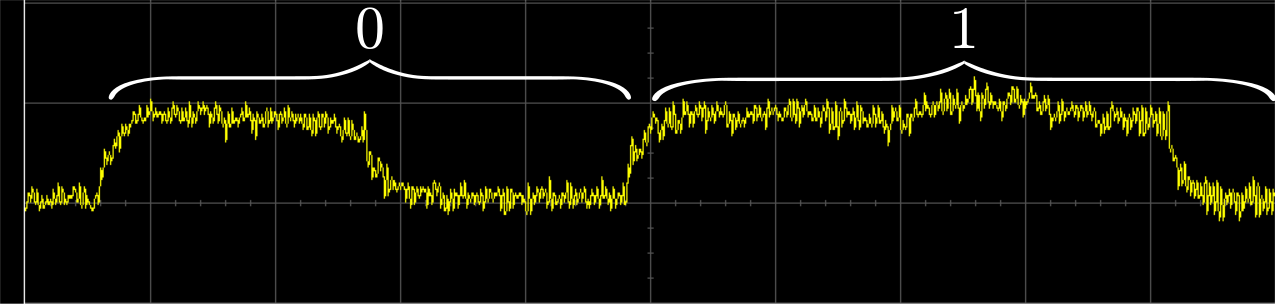
\includegraphics[width=\textwidth]{images/Power_attack}
  \caption{Messung des Stromverbrauchs für SPAs}
  \label{abb:power-attack}
\end{figure}

\subsection{Gegenmaßnahmen}
Um SPAs zu vermeiden, bieten sich Gegenmaßnahmen auf Hardware- und
Algorithmusseite an. Hardwareseitig kann man den Stromverbrauch
unabhängig von den ausgeführten Opereationen konstant halten. Zudem kann
man die Algorithmen so implementieren, dass ein keine bedingten Sprünge
in Abhängigkeit vom Geheimnis gibt. Außerdem können Dummy-Berechnungen
genutzt werden, um den Stromverbrauch und die Laufzeit  zu verrauschen.

\section{Differential Power Analysis (DPA)}
Eine aufwändigere, aber mächtigere Technik, um aus Power-Traces
Informationen über einen geheimen Schlüssel zu gewinnen, ist die
\emph{Differential Power Analysis (DPA)}. Um eine DPA durchführen zu
können, muss der Angreifer die Implementierung des Algorithmus kennen,
der auf dem Prozessor läuft. Auserdem braucht er eine möglichst große
Menge an Trace-Message-Paaren $(T_X, X)$, also jeweils den Stromverbrauch bei der
Entschlüsselung einer gegeben Nachricht (oder eines gegebenen
Chiffrats).
Ein Angreifer rät nun einen Teil $s$ des Geheimnis $S$. Dann simuliert
er den Algorithmus für alle $X$ und sortiert die Eingaben in zwei
Gruppen \calL, \calH, wobei
\begin{eqnarray*}
\calL & := &\{X| \texttt{Simulation mit $X$ hat einen niedrigen
  Stromverbrauch}\},\\
\calH & := &\{X| \texttt{Simulation mit $X$ hat einen hohen
  Stromverbrauch}\}.
\end{eqnarray*}
Anschließend betrachtet der Angreifer den durchschnittlichen
\textit{realen} Stromverbrauch beider Gruppen. War $s$ richtig geraten,
so sollte sich der reale Durschnittsverbrauch beider Gruppen stark
unterscheiden. Tut er dies nicht, so war $s$ wohl falsch geraten.

\subsection{Gegenmaßnahmen}
Um sich von DPAs zu schützen, kann man versuchen, den Stromverbrauch
durch zusätzliche Berechnungen zu verrauschen. Beispielsweise kann eine
Entschlüsselung vorgenommen werden mit $\plaint = \C^d = \frac{(R\cdot
  C)^d}{R^d}$, wobei $R$ zufällig gewählt wird.


%\section{theoretische Modelle}
